\section{Detekce}
\label{chap:detekce}

V tomto oddílu se zaměříme na první z problémů, který je způsobený tím, že v uspořádání na obr. \ref{fig:zakladni-schema} neměříme přímo stočení polarizace vzorkem, tj. neplatí vzorec \eqref{eqn:mustek-delta-beta}: $\Udif/2\Usum\neq\Delta\beta$.
Příčiny jsou dvě: zrcadla mezi vzorkem a můstkem měnící polarizaci, a nedokonalost vlnové destičky a děliče v můstku.

V tomto oddílu naplno využijeme formalismus \emph{Stokesových kovektorů} -- lineárních forem na prostoru Stokesových vektorů, které popisují detektory a složitější detekční systémy složené z detektorů a optických prvků -- rozvinutý v dodatku \ref{app:kovektory}.
Pomocí něj vysvětlíme podstatu problémů a popíšeme několik způsobů, jakými vliv zrcadel a nedokonalostí prvků kompenzovat.
Nakonec v oddílu \ref{chap:elipticita} popíšeme způsob využití Berekova kompenzátoru v můstku, který umožňuje současné měření stočení i elipticity.

Pro další použití v následujících oddílech na obr. \ref{fig:kovektor-ideal-mustek} vykreslujeme kovektory můstku s idealizovanými prvky (jako v oddílu \ref{chap:mustek-kap2}).
$\Dtks'$ značíme kovektory vzhledem ke světlu před děličem, $\Dtks''$ vzhledem ke světlu před destičkou.

\begin{figure}[htbp]
    \centering
    \begin{subfigure}{.35\textwidth}
        \centering
        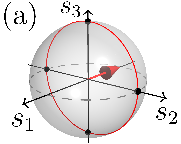
\includegraphics{./img/asy/pdf/kovek-2.pdf}
    \end{subfigure}%
    \begin{subfigure}{.34\textwidth}
        \centering
        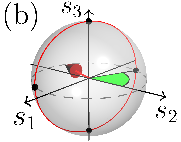
\includegraphics{./img/asy/pdf/kovek-3.pdf}
    \end{subfigure}%
    \begin{subfigure}{.3\textwidth}
        \centering
        \raisebox{-0.5cm}{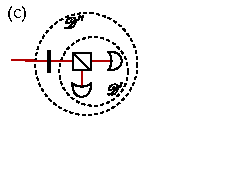
\includegraphics[scale=1.5,viewport=0 25 70 80,clip]{./img/svg/mustek-kovektory.drawio.pdf}}
    \end{subfigure}
    \caption{Stokesovy kovektory ideálního můstku. (a) Vzhledem ke světlu před děličem. (b) Vzhledem ke světlu před destičkou. Zeleně je vyznačen úhel $4\theta_{\lambda/2}$. (c) Ilustrace významu kovektorů $\Dtks'$ a $\Dtks''$ v optickém můstku.}
    \label{fig:kovektor-ideal-mustek}
\end{figure}

\subsection{Kompenzace nedokonalostí a zrcadel}
\label{chap:kompenzace}

Jedna z výhod formalismu Stokesových kovektorů je snadné uvažování o tom, jak se detekční aparatura chová při malých změnách (nedokonalostech) optických prvků.
Zaměříme se na tři druhy nedokonalostí, z nichž se nakonec jediná vyplatí kompenzovat -- nepřesné fázové zpoždění půlvlnné destičky.

Pro vyvažovací půlvlnnou destičku uvažujeme dva druhy nedokonalosti: rozdílnou propustnost obou módů a fázové zpoždění lišící se od přesné hodnoty $\pi/2$.
Kvůli symetrii však stále požadujeme, aby destička měla dvě navzájem kolmé optické osy -- dva vlastní módy navzájem ortogonálních lineárních polarizací.

Experimentálně bylo ověřeno, že polarizační dělič v optickém můstku (P2) vysoce kvalitně dělí svazek na dvě ortogonální lineární polarizace.
Při dopadu svazku na dělič je vertikální polarizace zcela odražena a v prošlém svazku je zastoupena tedy pouze horizontální polarizace.
Horizontální polarizace je ale také malou měrou odražena, takže odražený svazek není tvořen čistou vertikální polarizací. 
Nicméně každá z dvou ortogonálních polarizací je odražena mírně odlišným směrem a po určité dráze a průchodu čočkou se prostorově oddělí, takže detektorem B snímáme pouze průmět polarizace do vertikálního směru.

Vložením polarizátoru před dělič a jeho vhodným otáčením bylo možné ho zkřížit vzhledem k oběma ramenům (zvlášť) s extinkčním poměrem $I_\textrm{min}/I_\textrm{max}$ přibližně \num{1e-4}.
Díky tomu, že v každém rameni je polarizace takto kvalitně filtrovaná, se nijak neprojeví ani případná polarizační závislost detektorů.
Jediná nedokonalost zbytku můstku (nezahrnující půlvlnnou destičku) je tedy rozdílná citlivost obou ramen na příslušné lineární polarizace.
Ta je souhrnně způsobena jak rozdílnou propustností/odrazivostí děliče, tak nevyváženou citlivostí a zesílením obou detektorů.

Všechny tři zmíněné nedokonalosti uvažujeme zvlášť a zanedbáváme jejich vzájemné působení.
Nakonec se zaměříme na to, co se stane, když před můstek umístíme zrcadlo, které je nezbytné pro oddělení dopadajícího a odraženého svazku v reflexní geometrii, a pro vyvedení svazku ven z komory kryostatu v transmisní geometrii.


\subsubsection*{Nevyváženost ramen optického můstku}
Rozdíl citlivostí ramen je vyjádřen $\eta$, takže vzhledem ke světlu před děličem
\begin{subequations}
\begin{align}
    {\Dtks'}^\textrm{A}&=\frac{1-\eta}{2}(1, -1, 0, 0) \,,\\
    {\Dtks'}^\textrm{B}&=\frac{1+\eta}{2}(1, 1, 0, 0) \,,\\
    {\Dtks'}^\textrm{A-B}&=-(\eta, 1, 0, 0) \,,\\
    {\Dtks'}^\textrm{A+B}&=(1, \eta, 0, 0) 
\end{align}
\end{subequations}
a vzhledem ke světlu před destičkou
\begin{subequations}
\begin{align}
    {\Dtks''}^\textrm{A-B} &=-(\eta,\, \cos4\theta_{\lambda/2},\, \sin4\theta_{\lambda/2},\, 0) \,,\\
    {\Dtks''}^\textrm{A+B} &=(1,\, \eta\cos(\theta_{\lambda/2}),\, \eta\cos(\theta_{\lambda/2}),\, 0) \,.
\end{align}
\end{subequations}

Prvním z projevů je polarizační závislost součtového signálu (${d'_1}^\textrm{A+B}=\eta\neq0$).
To není velký problém, protože se ve vzorci $\Delta\beta=\Udif/2\Usum$ používá pouze pro normalizaci signálu, která lze určit i jiným způsobem (viz např. oddíl \ref{chap:elipticita}). 
Pro malé $\eta$ není od věci tento vliv ignorovat.

Druhou známkou nevyvážených ramen je nenulové  ${d'_0}^\textrm{A-B}$, které se projeví posunutím nulové kružnice jako na obr. \ref{fig:mustek-znazorneni-kovektoru}. 
Po průchodu ideální destičkou se pouze otočí v rovině $s_1s_2$.
Důležitým rysem je, že nulová kružnice je vždy kolmá na rovník lineárních polarizací, což znamená, že $\partial\Udif/\partial\chi = 0$, a tedy v měřeném signálu se neprojeví změny elipticity\footnote{Pokud do můstku vstupuje lineárně polarizované světlo.}.
I druhý projev neideálnosti optického můstku tedy v důsledku pouze mění konstantu úměrnosti, pro $\chi=0$ platí
\begin{equation}
    \textrm{d}\Udif = 2I \sqrt{1-\eta^2} \textrm{d}\beta \,,
\end{equation}
což pro malé $\eta$ ignorujeme.

\subsubsection*{Anizotropie amplitudové propustnosti destičky}
Jonesova a Muellerova matice destičky s přesným fázovým zpožděním $\pi/2$, ale rozdílnou propustností obou lineárních polarizací je (pro úhel natočení destičky $\theta_{\lambda/2}=0$)
\begin{align}
    \mathcal{T}_{\lambda/2} &= \begin{pmatrix} 1&0 \\ 0&-\eta \end{pmatrix} , &
    \M_{\lambda/2} &= \begin{pmatrix} \frac{1+\eta^2}{2}&\frac{1-\eta^2}{2}&0&0 \\ \frac{1-\eta^2}{2}&\frac{1+\eta^2}{2}&0&0 \\ 0&0&-1&0 \\ 0&0&0&-1 \end{pmatrix} ,
\end{align}
kde nedokonalost destičky je vyjádřena $\eta$ (ideální destička má $\eta=1$).
Akce takové Muellerovy matice je kombinace otočení o \SI{180}{\degree} a protáhnutí/posunutí kolem té stejné osy (viz oddíl \ref{chap:Stokes-Mueller})\footnote{To lze nahlédnout z toho, že lze Jonesovu matici psát jako součin unitární a pozitivně semi-definitní hermitovské matice, které spolu komutují: $\mathcal{T}_{\lambda/2} = \begin{pmatrix} 1&0\\0&-1 \end{pmatrix} \begin{pmatrix} 1&0\\0&\eta \end{pmatrix}$.} -- procházející lineárními polarizacemi ve směru optické osy $\theta_{\lambda/2}$.

Výsledkem je stejně jako v případě nevyvážených ramen posunutí nulové kružnice (${d''_0}^\textrm{A-B}\neq0$), které v souladu s diskuzí v předešlém oddílu pro malé $\eta$ ignorujeme.

\subsubsection*{Nepřesné fázové zpoždění destičky}
Jonesova a Muellerova matice je (pro $\theta_{\lambda/2}=0$)
\begin{align}
    \mathcal{T}_{\lambda/2} &= \begin{pmatrix} 1&0 \\ 0&-e^{i\delta} \end{pmatrix} , &
    \M_{\lambda/2} &= \begin{pmatrix} 1&0&0&0 \\ 0&1&0&0 \\ 0&0&-\cos\delta&\sin\delta \\ 0&0&-\sin\delta&-\cos\delta \end{pmatrix} ,
\end{align}
kde nedokonalost je vyjádřena dodatečným fázovým zpožděním $\delta$ (ideální destička má $\delta=0$).
Muellerova matice působí jako rotace o $\SI{180}{\degree}+\delta$ kolem osy vlastních módů.
Kvůli $\delta\neq0$ již nejsou obě osy destičky ekvivalentní.
Pozice destičky $\theta_{\lambda/2}$ a $\theta_{\lambda/2}+\SI{90}{\degree}$ tedy také nejsou ekvivalentní, odpovídají rotacím kolem té stejné osy o $\SI{180}{\degree}+\delta$, ale opačným směrem\footnote{Ekvivalentně s opačným znaménkem $\delta$.}.
Pozice $\theta_{\lambda/2}$ a $\theta_{\lambda/2}+\SI{180}{\degree}$ zůstávají nadále ekvivalentní.

Transformací kovektoru ideálního můstku ${\Dtks'}^\textrm{A-B}=(0, 1, 0, 0)$ neideální Muellerovou maticí $\M_{\lambda/2}$ je zachováno ${d''_0}^\textrm{A-B}=0$.
Oproti předchozím případům však již není zachovaná kolmost nulové kružnice a rovníku lineárních polarizací, tj. ${d''_3}^\textrm{A-B}\neq0$.
Ve sférických souřadnicích (${{d''_1}^\textrm{A-B}}^2+{{d''_2}^\textrm{A-B}}^2+{{d''_3}^\textrm{A-B}}^2=1$)
\begin{equation}
    {\Dtks''}^\textrm{A-B} \equiv (0,\, -\sin2\zeta_1\cos2\zeta_1,\, \cos2\zeta_1\cos2\zeta_2,\, \cos2\zeta_2) \,,
\end{equation}
kde jsme označili úhel průsečíku kružnice s rovníkem $2\zeta_1(\theta_{\lambda/2})$ a úhel vzájemného natočení $2\zeta_2(\theta_{\lambda/2})$, viz obr. \ref{fig:mustek-nedokonale-desticka}.

\begin{figure}[htbp]
    \centering
    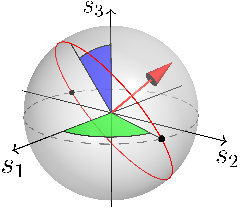
\includegraphics{./img/asy/pdf/kovek-4.pdf}
    \caption{Kovektor můstku s destičkou s nepřesným fázovým zpožděním (vzhledem ke světlu před destičkou). Zeleně úhel $2\zeta_1$, modře $2\zeta_2$.}
    \label{fig:mustek-nedokonale-desticka}
\end{figure}

Při vyvažování můstku (hledání $\theta_{\lambda/2}$ takového, aby $\Udif=0$) pro dané $\beta$ je nalezena pozice, pro kterou platí $\beta=\zeta_1(\theta_{\lambda/2})$.
Dosazením vyvažujícího $\zeta_1$ pak (viz \eqref{eqn:Stokes-diferencial} pro tvar $\textrm{d}\Stks$)
\begin{equation}
\label{eqn:mustek-s-elipticitou}
    \textrm{d}\Udif = {\Dtks''}^\textrm{A-B} \cdot \textrm{d}\Stks^\textrm{in} = 2I\left(\cos2\zeta_2 \textrm{d}\beta + \sin2\zeta_2\textrm{d}\chi\right)  \,.
\end{equation}

Zde však už narážíme na závažný problém: v měřeném signálu, který by měl odpovídat pouze otočení polarizace, se nám projevují i změny elipticity neznámým faktorem $\sin2\zeta_2$, který navíc závisí (i jeho znaménko) na $\beta$.
Řešení nám poskytuje skutečnost\footnote{Lze nahlédnout ze symetrie vůči obrácení točivosti světla či přímým výpočtem.}, že $\zeta_2$ je pro každé $\beta$ lichou funkcí nedokonalosti destičky $\delta$ -- mění znaménko při vyvážení polohami $\theta_{\lambda/2}$, resp. $\theta_{\lambda/2}+\SI{90}{\degree}$.
V praxi tedy měříme každé $\beta$ s oběma polohami destičky a bereme jejich aritmetický průměr
\begin{equation}
\label{eqn:mustek-kompenzace-desticek-prumer}
    \frac{1}{2}\left(\Udif^{\theta_{\lambda/2}}+\Udif^{\theta_{\lambda/2}+\SI{90}{\degree}}\right) = 2I\cos2\zeta_2 \textrm{d}\beta \,.
\end{equation}
Změny elipticity se odečetly a jediný zbývající vliv nedokonalosti je v dodatečném faktoru $\cos2\zeta_2$, který pro malé $\delta$ (a tedy malé $\zeta_2$) zanedbáváme.
Pokud není explicitně uvedeno jinak (v oddíle \ref{chap:elipticita}), provádíme tento krok vždy.
Ilustrace dat, která ukazují na nutnost provádět popsanou kompenzaci nedokonalého fázového zpoždění půlvlnné destičky, je na obr. \ref{fig:mustek-desticka-ilustrace}.
Potvrzením správnosti provedených kroků jsou ovšem až výsledky dosažené v kap.~\ref{chap:5}.

Poznamenejme, že uvedená procedura funguje pouze za předpokladu, že do destičky dopadá přibližně lineárně polarizované světlo, protože jenom pak jsou obě vyvažující polohy destičky posunuté přesně o \SI{90}{\degree}.
Při dopadu eliptického světla je situace výrazně složitější a dále se jí nezabýváme.

\begin{figure}[htbp]
    \centering
    \begin{subfigure}{.55\textwidth}
        \centering
        \includegraphics{./data/out/cofe-desticky-ilustrace.pdf}
    \end{subfigure}
    \begin{subfigure}{.43\textwidth}
        \centering
        \raisebox{0.1cm}{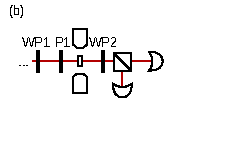
\includegraphics[width=2.7in]{./img/svg/cofe-rt.drawio.pdf}}
    \end{subfigure}
    \caption{Ilustrace potřeby provádět kompenzaci nepřesného fázového zpoždění vyvažovací půlvlnné fázové destičky. (a) Změřená data na $\lambda=\SI{810}{\nano\meter}$, která se liší pro dvě o \SI{90}{\degree} otočené polohy destičky (plnou a přerušovanou čarou). (b) Schéma experimentu: CoFe, pokojová teplota, transmisní geometrie, žádná zrcadla mezi vzorkem a můstkem.}
    \label{fig:mustek-desticka-ilustrace}
\end{figure}

\subsubsection*{Zrcadla}

Ve schématu experimentu na obr. \ref{fig:zakladni-schema} se v transmisní i reflexní geometrii vyskytují v dráze svazku mezi vzorkem a můstkem zrcadla.
Důvody jsou čistě geometrické, v reflexi je nutné odražený svazek prostorově oddělit od dopadajícího, v transmisi je nutné svazek po průchodu vzorkem vyvést v kolmém směru z kryogenní komory.
V obou případech svazek dopadá na zrcadlo přibližně pod úhlem \SI{45}{\degree}.

Experimentálně bylo zjištěno, že odraz od použitých zrcadel (stříbrné pokrytí s označením P01 od firmy Thorlabs) není izotropní.
Ve studovaném spektrálním rozsahu dosahuje světlo po jednom odrazu od zrcadla elipticity až \SI{10}{\degree}.
Zrcadlo modelujeme jako retardér s Jonesovou maticí
\begin{equation}
    \mathcal{T}_m = \begin{pmatrix} 1&0\\0&e^{i\delta_\textrm{m}} \end{pmatrix} .
\end{equation}

Vzhledem k nutnosti kompenzace nedokonalosti destičky, které vyžaduje, aby do ní vstupovala přibližně lineární polarizace, se úsilí k řešení tohoto problému soustředilo na fyzickou kompenzaci vlivu zrcadla na polarizaci detekovaného svaz\-ku pomocí vložení dalšího optického prvku, který působí inverzně.
Nejprve však uvedeme, jaký by mělo zrcadlo vliv na ideální můstek.
Mohli bychom zavádět kovektor $\Dtks'''$ vzhledem ke světlu před zrcadlem, který by měl stejný tvar jako \eqref{eqn:mustek-s-elipticitou}, ale s rozdílnou závislostí $\zeta_1$ a $\zeta_2$ na $\theta_{\lambda/2}$.
Pro kvalitativní pochopení je v tomto případě ale názornější zůstat u $\Dtks''$ a namísto kovektoru zrcadlem zobrazit vstupní Stokesovy vektory.

Pro ideální můstek je nulová kružnice $\Dtks''$ tvořena poledníkem, který je během vyvažování otáčen kolem osy $s_3$ tak, aby procházel bodem odpovídajícím vstupní polarizaci.
Zrcadlo je retardér s osou podél $s_1$, takže podél ní otočí rovník lineárních polarizací o úhel $\delta_\textrm{m}$.
Zároveň se Stokesovým vektorem však musíme zobrazit i jeho diferenciál (změna $\beta$ před zrcadlem se projeví i změnou $\chi$ za zrcadlem).
Viz obr.~\ref{fig:mustek-zrcadlo-data}~(a).

Ze vzájemné orientace nulové kružnice a diferenciálu Stokesova vektoru lze graficky určit, jakými faktory se do měřeného signálu promítne $\textrm{d}\beta$ a $\textrm{d}\chi$.
Pro význačné $\beta$ lze odečíst přímo z obrázku \ref{fig:mustek-zrcadlo-data} (a)
\begin{align}
    \textrm{d}\Udif(\beta=\SI{0}{\degree}) &= 2I\left(\cos(\delta_\textrm{m})\textrm{d}\beta + \sin(\delta_\textrm{m})\textrm{d}\chi\right) \,,\\
    \textrm{d}\Udif(\beta=\SI{90}{\degree}) &= 2I\left(\cos(\delta_\textrm{m})\textrm{d}\beta - \sin(\delta_\textrm{m})\textrm{d}\chi\right) \,,\\
    \textrm{d}\Udif(\beta=\SI{45}{\degree}) &= 2I\textrm{d}\beta \,, \label{eqn:must-zrc-1}\\
    \textrm{d}\Udif(\beta=\SI{135}{\degree}) &= 2I\textrm{d}\beta \,. \label{eqn:must-zrc-2}
\end{align}

Zde je jasně vidět původ prvního popsaného problému, kterým trpí např. data na obr. \ref{fig:g-uvod-data} (a), totiž že změřená data pro $\beta$ a $\beta+\SI{90}{\degree}$ jsou zcela odlišná.
Problém se zrcadly dlouho unikal pozornosti, především z toho důvodu, že jsou to právě polarizace $\beta=\SI{0}{\degree}, \SI{90}{\degree}$, které jsou nejvíce ovlivněny, zatímco $\beta=\SI{45}{\degree}, \SI{135}{\degree}$ jsou ovlivněny jen minimálně.
Na první pohled by se mohlo zdát, že s- a p-polarizace jsou přece na zrcadlech odraženy beze změny\ldots

Náhodou je tento neduh zdánlivě ``vyřešen'', pokud světlo po odrazu od vzorku projde ještě jednou půlvlnnou destičkou WP1, jako v \cite{wohlrathMagnetooptickaCharakterizaceSpintronickych2018,kubascikMagnetooptickeStudiumAntiferomagnetickych2019,kimakOptickaSpektroskopieAntiferomagnetu2019}.
Pak je pro všechna $\beta$ následně měřen stejný mix stočení a elipticity, takže vypadají věrohodně.

\begin{figure}[htbp]
    \centering
    \begin{subfigure}{.6\textwidth}
        \centering
        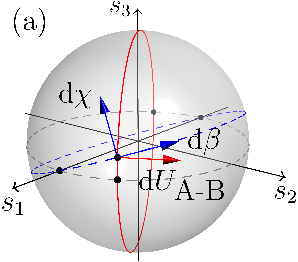
\includegraphics{./img/asy/pdf/kovek-5.pdf}
    \end{subfigure}
    \begin{subfigure}{.3\textwidth}
        \centering
        \raisebox{1.4cm}{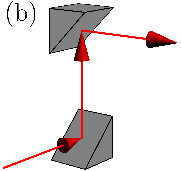
\includegraphics{./img/asy/pdf/zrcadla.pdf}}
    \end{subfigure}
\caption{(a) Vliv zrcadla mezi vzorkem a optickým můstkem. Je znázorněn Stokesův kovektor ${\Dtks''}^\textrm{A-B}$ vzhledem ke světlu před můstkem (červeně) a rovník lineárních polarizací po odrazu zrcadlem (modře). Zároveň je naznačen vzájemný směr diferenciálů, který určuje kofaktory stočení a elipticity v měřeném signálu. (b) Zkřížená zrcadla, která společně působí přibližně jako neutrální prvek.}
    \label{fig:mustek-zrcadlo-data}
\end{figure}

Nejjednodušší způsob, jakým zanesenou elipticitu vlivem zrcadla kompenzovat, je přidat ještě jedno identické zrcadlo, ve kterém je role s- a p- polarizace prohozena (odraz nahoru a do strany jako na obr. \ref{fig:mustek-zrcadlo-data} (b).
Obě polarizace pak po dvou odrazech nabydou stejného fázového faktoru.
Dvojici zrcadel v následujícím textu nazýváme \emph{zkřížená zrcadla} a chovají se z hlediska polarizace jako neutrální prvek.
Tato jejich optická neutralita byla experimentálně ověřena v celém používaném spektrálním rozsahu (460--\SI{1600}{\nano\meter}): elipticita lineárně polarizovaného světla po průchodu zkříženými zrcadly nepřesahuje \SI{3}{\degree}, a to poněkud překvapivě i v případě, kdy je jedno ze zrcadel uvnitř kryostatu zchlazené na teplotu \SI{15}{\kelvin} a druhé je na pokojové teplotě.
Trik zkřížených zrcadel je použit ve všech experimentech uvedených v kap.~\ref{chap:5}.

Nicméně experimentálně byla v rámci řešení této práce otestována ještě jedna metoda kompenzace vlivu odrazu na zrcadle, kterou zde popíšeme -- pomocí Berekova kompenzátoru.
Berekův kompenzátor je laditelný retardér a je proto možné jeho správným nastavením zrcadlo kompenzovat.
Jedinou komplikací je právě nutnost nalézt jeho správné nastavení.
To jsme provedli dvěma způsoby.

První způsob, který označujeme jako \emph{statický}, se snaží nastavit fixní polohu, která zrcadlo zcela kompenzuje pro všechna $\beta$.
Procedura je zdlouhavá a probíhá iteračně: nejdříve je správně zorientovaná optická osa Berekova kompenzátoru, a poté nastavené správné fázové zpoždění, zatímco je pomocí rotačního analyzátoru za kompenzátorem měřena elipticita pro vybrané hodnoty vstupního $\beta$ (především \SI{45}{\degree} a $\SI{135}{\degree}$).
Správného nastavení je dosaženo, když je elipticita za kompenzátorem nulová pro všechna $\beta$ -- každá lineární polarizace před zrcadlem je lineární i za kompenzátorem.

Druhý způsob označujeme jako \emph{dynamický}, protože neaspiruje na kompenzaci vlivu zrcadla, ale je nastavován pro každé $\beta$ zvlášť.
Princip je založen na tom, že není striktně vzato nutné zrcadlo kompenzovat. Vždyť \eqref{eqn:must-zrc-1}, \eqref{eqn:must-zrc-2} jsou v pořádku i se zrcadlem -- můstek dokáže měřit čisté stočení $\textrm{d}\beta$, i když do něj vstupuje eliptické světlo.
Toto rozvolnění ubírá jeden stupeň volnosti Berekova kompenzátoru, který je nutno přesně nastavit, a tím proceduru výrazně usnadňuje.
Ve dvoudimenzionálním stavovém prostoru Berekova kompenzátoru (poloha osy a fázové zpoždění) existuje pouze jeden bod, který ho správně nastaví staticky, ale celá křivka, která ho nastaví dynamicky.

Cílem je nastavit pro každé $\beta$ Berekův kompenzátor tak, aby se vynuloval koeficient $\textrm{d}\chi$ v $\Udif$ a platilo prosté $\textrm{d}\Udif=2I\textrm{d}\beta$.
Za účelem zpětné vazby byl využit PEM umístěný před vzorek, viz obr. \ref{fig:berek} (a).
Amplituda fázového zpoždění $\delta_\textrm{PEM}$ byla nastavována v rozsahu hodnot přibližně 0--\SI{10}{\degree}.
Osa PEMu by měla být ideálně otočená o \SI{45}{\degree} oproti $\beta$, ale není to nutností.
Pro malé zpoždění dochází totiž pouze k periodickému kmitání $\chi$ s frekvencí $\omega_\textrm{PEM}$, zatímco $\beta$ kmitá s amplitudou až v druhém řádu $\propto\delta_\textrm{PEM}^2$ a s frekvencí $2\omega_\textrm{PEM}$ (viz obr. \ref{fig:UH-Mueller} (a)), a toto platí pro všechny lineární polarizace neprocházející přímo osou PEMu.
Rozdílové napětí na frekvenci $\omega_\textrm{PEM}$ by tedy mělo být úměrné koeficientu $\textrm{d}\chi$.

Dynamické nastavení tedy spočívá v současném/střídavém točení vyvažovací destičky, osy a zpoždění kompenzátoru, zatímco na dvou lock-inech jsou sledovány hodnoty $\Udif(\omega=0)$ a $\Udif(\omega=\omega_\textrm{PEM})$ s cílem obě současně vynulovat.
Tímto způsobem jsme se mimoděk vyhnuli problému s nedokonalými destičkami, protože nulovaný koeficient $\textrm{d}\chi$ není specifický pro zrcadla, ale zahrnuje v sobě celou detekční aparaturu.
S dynamickým Berekovým kompenzátorem není třeba měřit MO signál pro obě polohy vyvažovací destičky.

Oběma způsoby je Berekův kompenzátor vždy nastaven do polohy jedné ze dvou tříd lišících se v tom, jestli se dvojice zrcadlo--kompenzátor dohromady chová jako neutrální prvek (``nedotáčivý mód'', $\delta_m+\delta_B=0$) či půlvlnná destička (``přetáčivý mód'', $\delta_m+\delta_B=\pi$).

Obě metody nastavení byly vyzkoušeny na vzorku CoFe v transmisní geometrii při pokojové teplotě (bez vakuové komory kryostatu), viz obr. \ref{fig:berek} (b).
Z obrázku je patrné, že obě metody kompenzace fungují spolehlivě.
Při měření byly mezi vzorkem a můstkem umístěny dvě zrcadla jako na obr. \ref{fig:zakladni-schema}.
Zrcadla byla umístěna paralelně, takže se dá očekávat, že se chovají jako retardér s dvojnásobným fázovým zpožděním.
Dále jsme se kompenzací zrcadel Berekovým kompenzátorem nevěnovali.

\begin{figure}[htbp]
    \centering
    \begin{subfigure}{.48\textwidth}
        \centering
        \raisebox{0.9cm}{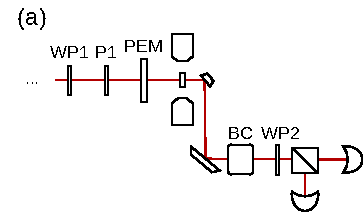
\includegraphics{./img/svg/schema-pem.drawio.pdf}}
    \end{subfigure}
    \begin{subfigure}{.48\textwidth}
        \centering
        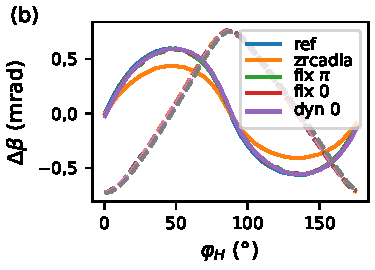
\includegraphics{./data/out/pem-data.pdf}
    \end{subfigure}
    \caption{(a) Schéma pro testování Berekova kompenzátoru (BC). V případě dynamického nastavení je před vzorek umístěn PEM. 
    (b) Změřená data CoFe při pokojové teplotě, $\lambda=\SI{1050}{\nano\meter}$, po symetrizaci v poli a filtraci frekvencí $2\beta$ (viz oddíl \ref{chap:anizotropie-MLD}). Polarizace $\beta=\SI{0}{\degree}$ (plná čára), $\beta=\SI{45}{\degree}$ (přerušovaná čára). Pro porovnání jsou zobrazena i data měřená bez zrcadel (ref) a s nimi. fix/dyn značí fixní/dynamické nastavení, $0/\pi$ značí nedotáčivý/přetáčivý mód. Vykreslená data nejsou přímo měřená, ale je z nich vybraná frekvence $2\beta$ (viz oddíl \ref{chap:anizotropie-MLD}).}
    \label{fig:berek}
\end{figure}

\subsection{Současné měření elipticity}
\label{chap:elipticita}

Měření MO dat pro dvě polohy vyvažovací destičky je časově náročné a v jistém smyslu slova zahazuje polovinu dat.
Metoda kompenzace pomocí \eqref{eqn:mustek-kompenzace-desticek-prumer} se zajímá pouze o průměr signálů v obou polohách a nebere v potaz jejich rozdíl, který v sobě nese informaci o elipticitě -- druhý člen \eqref{eqn:mustek-s-elipticitou} $\sin2\zeta_2 \textrm{d}\chi$.
Změnu elipticity od vzorku $\Delta\chi$ však nelze takto jednoduše ze signálu extrahovat, protože je vážena neznámým faktorem $\sin2\zeta_2$, který je navíc malý.

Vyvinuli jsme proto metodu charakterizace Stokesova kovektoru můstku, která nám dodá neznámé faktory stočení i elipticity v měřeném signálu.
Základem metody je studium měřeného signálu pro všechny vstupní lineární polarizace.
Pokud vyvážíme můstek pro vstupní $\beta_0$ a celkový kovektor označíme $\Dtks^{\beta_0}$, pak
\begin{equation}
\label{eqn:charakterizace-kovektoru-beta}
\begin{split}
    \Udif &= \Dtks^{\beta_0} \cdot \Stks \\ &= I \left[d^{\beta_0}_0+ \cos2\chi\left(d^{\beta_0}_1 \cos2\beta + d^{\beta_0}_2 \sin2\beta  \right) + d^{\beta_0}_3 \sin2\chi  \right] \\
          &\equiv I \left[ d^{\beta_0}_0+ \cos2\chi \left(d^{\beta_0}_\perp \sin \left( 2\psi^{\beta_0} - 2\beta \right) \right) + d^{\beta_0}_3 \sin2\chi \right] \,,
\end{split}
\end{equation}
kde jsme zavedli cylindrické souřadnice kovektoru pomocí $d^{\beta_0}_\perp$ a $\psi^{\beta_0}$.
Ve vyváženém můstku platí (pro $\chi=0$)
\begin{equation}
    d^{\beta_0}_0 + d^{\beta_0}_\perp \sin \left( 2\psi^{\beta_0} - 2\beta_0 \right) = 0 \,.
\end{equation}

Výpočtem gradientu v tomto vyváženém bodě pak dostaneme pro malé změny (způsobené vzorkem) polarizačního stavu (a intenzity)
\begin{equation}
    \textrm{d}\Udif(\beta_0) = 2I \left(\sqrt{1 - \left(\frac{d^{\beta_0}_0}{d^{\beta_0}_\perp}\right)^2} \textrm{d}\beta + d^{\beta_0}_3 \textrm{d}\chi  \right) \,.
\end{equation}

Pokud dokážeme charakterizovat všechny složky kovektoru, dokážeme určit oba kofaktory $\textrm{d}\beta$ i $\textrm{d}\chi$.
Po provedení dvou měření, ve kterých se kofaktory liší, je pak možné určit stočení i elipticitu od vzorku.

\subsubsection*{Charakterizace kovektoru}

Předkládaná metoda charakterizace visí na předpokladu, že jsme schopni do můstku svítit světlem s libovolně natočenou lineární polarizací \beta.
V praxi to provádíme tak, že s danou polarizací svítíme na vzorek a předpokládáme, že se po průchodu/odrazu příliš nezmění.
V prvním ze zkušebních experimentů -- tenký film CoFe v transmisní geometrii při pokojové teplotě -- byl tento předpoklad experimentálně ověřen.
V druhém -- FeRh v transmisní geometrii při \SI{420}{\kelvin} -- nebyl ověřen, ale vzhledem k úhlu dopadu $<\SI{0.5}{\degree}$ mu stejně věříme.
S tímto předpokladem lze složky $d^{\beta_0}_0, d^{\beta_0}_1, d^{\beta_0}_2$ snadno určit z $\beta$-závislosti \eqref{eqn:charakterizace-kovektoru-beta}.


Poslední složku $d^{\beta_0}_3$ nelze určit přímo, aniž bychom dokázali definovaně měnit vstupní elipticitu.
K jejímu určení je potřeba splnit dvojici předpokladů.
Zaprvé již zmíněný experimentálně ověřený fakt, že oba z detektorů lze vynulovat vhodnou lineární polarizací před děličem.
To znamená, že vzhledem ke světlu před můstkem předpokládáme\footnote{Vyjádřenou v souřadné soustavě děliče, takže $d'_2=0$ nezahrnuje předpoklad přesné shodnosti se souřadnou soustavou světla před můstkem.}

\begin{subequations}
\label{eqn:kovektory-det-elipticita}
\begin{align}
    {\Dtks'}^\textrm{A} &= {d'}^{\textrm{A}}_0(1, -1, 0, 0) \,,\\
    {\Dtks'}^\textrm{B} &= {d'}^\textrm{B}_0(1, 1, 0, 0) \,.
\end{align}
\end{subequations}

Druhým předpokladem, který zřejmě není splněn zcela, je alespoň přibližná unitarita celé soustavy optických prvků před děličem (zachování intenzity při průchodu přes zrcadlo, destičku, \ldots).
Pak totiž 3-kovektor $(d_1, d_2, d_3)$ zachovává svoji normu a vzhledem ke světlu od vzorku lze třetí složku (až na znaménko) určit pomocí
\begin{equation}
{d_1^\textrm{A/B}}^2 +  {d_1^\textrm{A/B}}^2 + {d_3^\textrm{A/B}}^2 = {d_0^\textrm{A/B}}^2 \,,
\end{equation}
pokud změříme průběh napětí na každém detektoru zvlášť
\begin{equation}
    U^\textrm{A/B}(\beta) = I \left( d^\textrm{A/B}_0 + d^\textrm{A/B}_1 \cos2\beta + d^\textrm{A/B}_2 \sin2\beta  \right) \,.
\end{equation}

Z $\beta$-závislosti napětí na obou detektorech lze klasicky určit jejich $d_0, d_1, d_2$, ale díky unitaritě lze navíc určit absolutní hodnotu $d_3$:
Znaménko $d_3$ touto metodou určit nedokážeme.
Nicméně vzhledem k tomu, že 3-kovektory obou detektorů před můstkem \eqref{eqn:kovektory-det-elipticita} mají opačnou orientaci, musí i před celou soustavou mít opačné znaménko: $d^\textrm{A}_3 \times d^\textrm{B}_3 < 0$.

Když máme určeny kovektory jednotlivých detektorů, vrátíme se k rozdílovému napětí $\Udif$.
Předpokládáme, že je dáno jednoduše rozdílem napětí na obou detektorech, avšak každé může být zesíleno mírně odlišným faktorem.
V každém případě by pořád mělo platit
\begin{equation}
    \frac{d^\textrm{A-B}_3}{d^\textrm{A-B}_\perp} = \frac{d^\textrm{A}_3}{d^\textrm{A}_\perp} = \frac{d^\textrm{B}_3}{d^\textrm{B}_\perp} \,,
\end{equation}
takže jsme již schopní určit $d^\textrm{A-B}_3$.
Hodnoty pro A a B by měly při splnění všech předpokladů být stejné, ale v praxi se samozřejmě mírně liší.
Pak bereme nějakou jejich vhodnou kombinaci, my jsme zvolili bez dalšího zdůvodnění geometrický průměr.

Pokud nelpíme na určení absolutního znaménka elipticity, stačí znát pou\-ze relativní znaménko $d_3$ mezi různými vyváženími můstku, tj. mezi různými $\beta_0$.
Absolutní hodnota znaménka pak už jen udává, jestli měříme $+\Delta\chi$ či $-\Delta\chi$.
Relativní znaménko lze spolehlivě určit z přibližného teoretického výpočtu, viz např. oddíl o kompenzaci zrcadel výše ($\beta_0=\SI{0}{\degree}$ a $\beta_0=\SI{90}{\degree}$ mají opačná znaménka).

Přesto jsme však při zkušebním experimentu s CoFe provedli pokus o jeho experimentální určení.
Postup je následující.
Nejdříve je vyvážen můstek pro dané $\beta_0$.
Dále je před celou měřící soustavu (nejlépe za vzorek, v našem případě před vzorek) umístěna čtvrtvlnná destička s definovanou osou zorientovanou přibližně ve směru $\beta_0$.
Je nalezena přibližná poloha čtvrtvlnné destičky, která vyvažuje můstek (teoreticky by to měla být přesně poloha, kdy její osa splývá s $\beta_0$).
Destička je drobně vychýlena do definovaného \emph{kladného} směru a je zaznamenáno znaménko $\Udif$.
Protože toto kladné vychýlení zanáší pro všechna $\beta_0$ malou elipticitu stejného znaménka, jsou tím relativní znaménka určena.
Pro určení absolutního znaménka by pak stačilo zjistit, zda je definovaná osa destičky pomalá či rychlá.
Čtvrtvlnná destička je samozřejmě opět vyjmuta pro samotné měření.

Ve všech vzorcích pro $\Udif$ jsme explicitně psali faktor $I$, protože pochází ze Stokesova vektoru a ne kovektoru.
Při měření $\beta$-závislosti napětí je ale již zahrnut, což nám usnadňuje práci.
S fitovanými parametry $a$ v $\beta$-závislostech
\begin{subequations}
\begin{align}
    U^\textrm{A}(\beta) &= a^\textrm{A}_0 + a^\textrm{A}_1 \cos2\beta + a^\textrm{A}_2 \sin2\beta \,,\\
    U^\textrm{B}(\beta) &= a^\textrm{B}_0 + a^\textrm{B}_1 \cos2\beta + a^\textrm{B}_2 \sin2\beta \,,\\
    U^\textrm{A-B}(\beta) &= a^\textrm{A-B}_0 + a^\textrm{A-B}_1 \cos2\beta + a^\textrm{A-B}_2 \sin2\beta
\end{align}
\end{subequations}
jsou pak kofaktory stočení a elipticity (s geometrickým průměrem faktorů od A a B)
\begin{equation}
\label{eqn:elipticita-kofaktory}
\textrm{d}\Udif = \sqrt{1-\frac{{a^\textrm{A-B}_0}^2}{{a^\textrm{A-B}_1}^2+{a^\textrm{A-B}_2}^2}}\textrm{d}\beta 
+ \sqrt[4]{\left(\frac{{a^\textrm{A}_0}^2}{{a^\textrm{A}_1}^2+{a^\textrm{A}_2}^2}-1 \right)\left(\frac{{a^\textrm{B}_0}^2}{{a^\textrm{B}_1}^2+{a^\textrm{B}_2}^2}-1 \right)}\textrm{d}\chi \,.
\end{equation}
Změření celé závislosti $U^\textrm{A-B}(\beta)$ vyžaduje změnu zesílení, aby nedošlo k překročení měřícího rozsahu lock-inů.
Proto používáme \eqref{eqn:elipticita-kofaktory} pouze k určení poměru obou kofaktorů
\begin{equation}
    \textrm{d}\Udif = g \left( \textrm{d}\beta + \frac{\sqrt[4]{\left(\frac{{a^\textrm{A}_0}^2}{{a^\textrm{A}_1}^2+{a^\textrm{A}_2}^2}-1 \right)\left(\frac{{a^\textrm{B}_0}^2}{{a^\textrm{B}_1}^2+{a^\textrm{B}_2}^2}-1 \right)}}{\sqrt{1-\frac{{a^\textrm{A-B}_0}^2}{{a^\textrm{A-B}_1}^2+{a^\textrm{A-B}_2}^2}}}\textrm{d}\chi \right) \,.
\end{equation}
Kofaktor stočení $g$ určíme přímo: změříme několik $\beta$ v malém okolí $\beta_0$ (např. $\pm\SI{1}{\degree}$ a body proložíme přímkou; $g$ je pak její směrnicí.

Pro přesné určení obou kofaktorů je žádoucí, aby měly oba přibližně stejnou velikost.
Toho lze docílit vložením Berekova kompenzátoru mezi vyvažovací půlvlnnou destičku a polarizační dělič v optickém můstku.
Osa kompenzátoru je nastavena diagonálně vzhledem k dvoum hlavním módům děliče a fázové zpoždění je nastaveno $\pi/4$.

